\section{10362 - Trains}
\textbf{Problema:} Dado un conjunto de rutas de tren, determinar las conexiones
``\'optimas'' entre dos estaciones dadas. Una conexi\'on $c$ es \'optima
si se cumple lo siguiente:

\begin{enumerate}
\item[(A)] No hay una conexi\'on $c'$ que salga m\'as tarde y llegue m\'as temprano o a la misma hora que $c$.
\item[(B)] No hay una conexi\'on $c'$ que salga a la misma hora y llegue m\'as temprano que $c$.
\end{enumerate}

\subsection{Resoluci�n}

La idea del algoritmo propuesto es primero encontrar los caminos m\'as
cortos (en minutos) entre la estaci\'on de origen y la estaci\'on de
destino. Estos cumplen con la condici\'on (B). Una vez hecho esto,
determinar cu\'ales de ellos cumplen con la condici\'on (A).

El problema de encontrar los caminos m\'as cortos se modela como un
problema de camino m\'inimo.

\subsubsection{Descripci\'on del grafo asociado al problema}
En primer lugar, construimos un grafo orientado con pesos en los ejes
$G = (V,E)$, cuyos nodos
representan una estaci\'on y una hora del d\'ia, y cuyos ejes representan
una manera de llegar de una pareja estaci\'on/hora a otra. El grafo
contiene los siguientes nodos:

$(n,h)\in V \longleftrightarrow$ existe un tren que pasa por la estaci\'on
$n$ a las $h$ horas $(h \in [\text{0:00}..\text{23:59}])$

%%$FINAL \in V$

Adem\'as, hay un eje desde $(n_1,h_1)$ hasta $(n_2,h_2) \longleftrightarrow$ se cumple alguno de los dos casos siguientes:
\begin{enumerate}
\item Existe un tren que pasa por $n_1$ a las $h_1$ y cuya siguiente parada es en $n_2$ a las $h_2$ (sin pasar por estaciones intermedias).
\item $n_1 = n_2$ (es la misma estaci\'on) y $h_2$ es el horario que sigue a $h_1$ en orden cronol\'ogico, sin pasar por horas intermedias.
\end{enumerate}
%\begin{enumerate}
%\item existe una ruta que permite tomar un tren en $n_1$ a las $h_1$ y llegar a $n_2$ a las $h_2$.
%\item $n_1=n_2 \wedge h_1<h_2 \wedge \nexists h_3 / (n_1,h_3) \in V \wedge h_1 < h_3 < h_2$
%\item $n_1=n_2 \wedge h_1 > h_2 \wedge \nexists h_3 / (n_1,h_3) \in V \wedge ( h_1 < h_3 \vee h_3 < h_2)$
%\end{enumerate}

Los ejes que resultan de la primera condici\'on tienen como peso asociado el tiempo de viaje.
Si bien se conoce la hora del d\'ia asociada a cada nodo, es necesario conocer el peso
expl\'icitamente, porque el tiempo de viaje entre dos estaciones {\em puede} ser mayor a un d\'ia.

Los ejes que resultan de la segunda condici\'on representan la posibilidad de quedarse
en una estaci\'on y esperar el pr�ximo tren. En este caso, el peso del eje es la diferencia
entre $h_2$ y $h_1$. Cuando decimos que $h_2$ es el horario que sigue a $h_1$
``en orden cronol\'ogico'', tambi\'en hay que considerar que $h_1$ puede ser
el \'ultimo tren del d\'ia y $h_2$ el primer tren del d\'ia siguiente. En ese caso
el peso del eje es la diferencia m\'odulo 24 horas.

%TODO: esto hay que explicarlo mas y/o mejor?
El grafo descripto modela el problema porque una conexi�n permite
llegar de una estaci\'on/hora a otra si y s\'olo si existe
un camino entre los dos nodos correspondientes del grafo, de manera tal que el tiempo que
tarda la conexi\'on es el peso del camino. Esto es porque o bien el
camino es una ruta directa sin cambiar de tren (en cuyo caso, por
los ejes del caso $1$, hay un camino en el grafo con el peso apropiado),
o bien la conexi�n usa fragmentos de varias rutas. Para hacer esto,
es necesario esperar cierto tiempo en una estaci\'on para cambiar de tren.
El tiempo de espera debe ser contabilizado
tambi�n, lo que se logra con los ejes del caso $2$. Si es posible hacer
una combinaci�n sin esperar, es porque se llega a una estaci\'on a la misma
hora en que sale el siguiente tren. Esto no representa un problema
porque el enunciado indica que el tiempo necesario para realizar la conexi�n
est� incorporado en los horarios de los trenes. Por el caso $1$, ese nodo
tiene ambos ejes, y el camino es realizable. De manera similar
se ve lo inverso, es decir que cualquier camino en el grafo representa
una conexi\'on v\'alida.

Notar que, en el primer caso, se agrega un eje s\'olo cuando la ruta no pasa por estaciones
intermedias. De manera similar, en el segundo caso, se agrega un eje de $(n,h_1)$ a $(n,h_2)$
s\'olo cuando no existe un horario $h_3$ entre $h_1$ y $h_2$.
Es decir, el grafo se construye {\em sin} hacer la clausura transitiva
de los ejes. No es necesario agregar los ejes restantes, porque lo que
importa es la duraci\'on en minutos de los caminos, y todos
los caminos posibles est\'an dados precisamente la clausura transitiva
de los ejes.
La ventaja es que de esta manera la cantidad de ejes del grafo
es lineal en el tama\~no de la entrada.

\subsubsection{B\'usqueda de los caminos m\'inimos}

Una vez que se tiene el grafo descripto en la secci\'on anterior,
el objetivo es determinar las duraciones de las conexiones \'optimas.
Las conexiones \'optimas deben ser caminos m�nimos entre nodos de la estaci\'on de origen
($src$) y la estaci\'on de destino ($dst$). Si no se tratara de caminos m�nimos, ser�a posible
encontrar un camino que sale a la misma hora y llega antes (de menor duraci\'on, y por
lo tanto de menor peso), y la conexi�n no ser�a \'optima por no cumplir con
la condici\'on (B).

El primer objetivo es determinar, para cada nodo $(src,h)$ el peso del
camino m\'inimo hasta alg\'un nodo $(dst,h')$.
Los pesos de los ejes son todos positivos, por lo cual es relativamente
sencillo convertir este problema en un problema de camino m\'inimo
{\em single-source}, para as\'i poder aplicar el algoritmo de Dijkstra.

Para convertir el problema, se agrega un nodo $\textsc{final}$ y, para
cada nodo de la forma $(dst,h)$, un eje de peso 0 hacia el nodo $\textsc{final}$.
Por \'ultimo, se considera el grafo $G'$ que resulta de invertir
todos los ejes en $G$ y se calculan los caminos m\'inimos en $G'$ desde
$\textsc{final}$ hasta todos los dem\'as nodos, usando el algoritmo
de Dijkstra.

Cada uno de los caminos m\'inimos encontrados en $G'$ que terminan en nodos
de la forma $(src,h)$, corresponden a alg\'un camino en $G$ que empieza en $(src,h)$,
llega hasta alg\'un nodo $(dst,h')$, y por \'ultimo llega a $\textsc{final}$
mediante un eje de peso 0. El peso del camino correspondiente en $G$ es m\'inimo
y es el mismo que el encontrado en $G'$.

%Por otro lado, todas los nodos cuya estaci\'on es la de destino, tienen un eje de costo $0$ con el nodo $FINAL$.

Como observaci\'on adicional, dado que lo que se busca son caminos
m\'inimos, si una estaci\'on $n$ tiene un \'unico horario $h$ en el que salen o
llegan trenes, durante la construcci\'on del grafo $G$ no se agrega el autoeje
$(n,h)$, porque este eje tiene peso de 24 horas y obviamente nunca es conveniente
(existe un camino desde $v$ hasta $w$ que pasa por dicho eje si y s\'olo si existe
un camino de $v$ a $w$ de menor peso que no lo utiliza).

\begin{figure}[H]
\centering
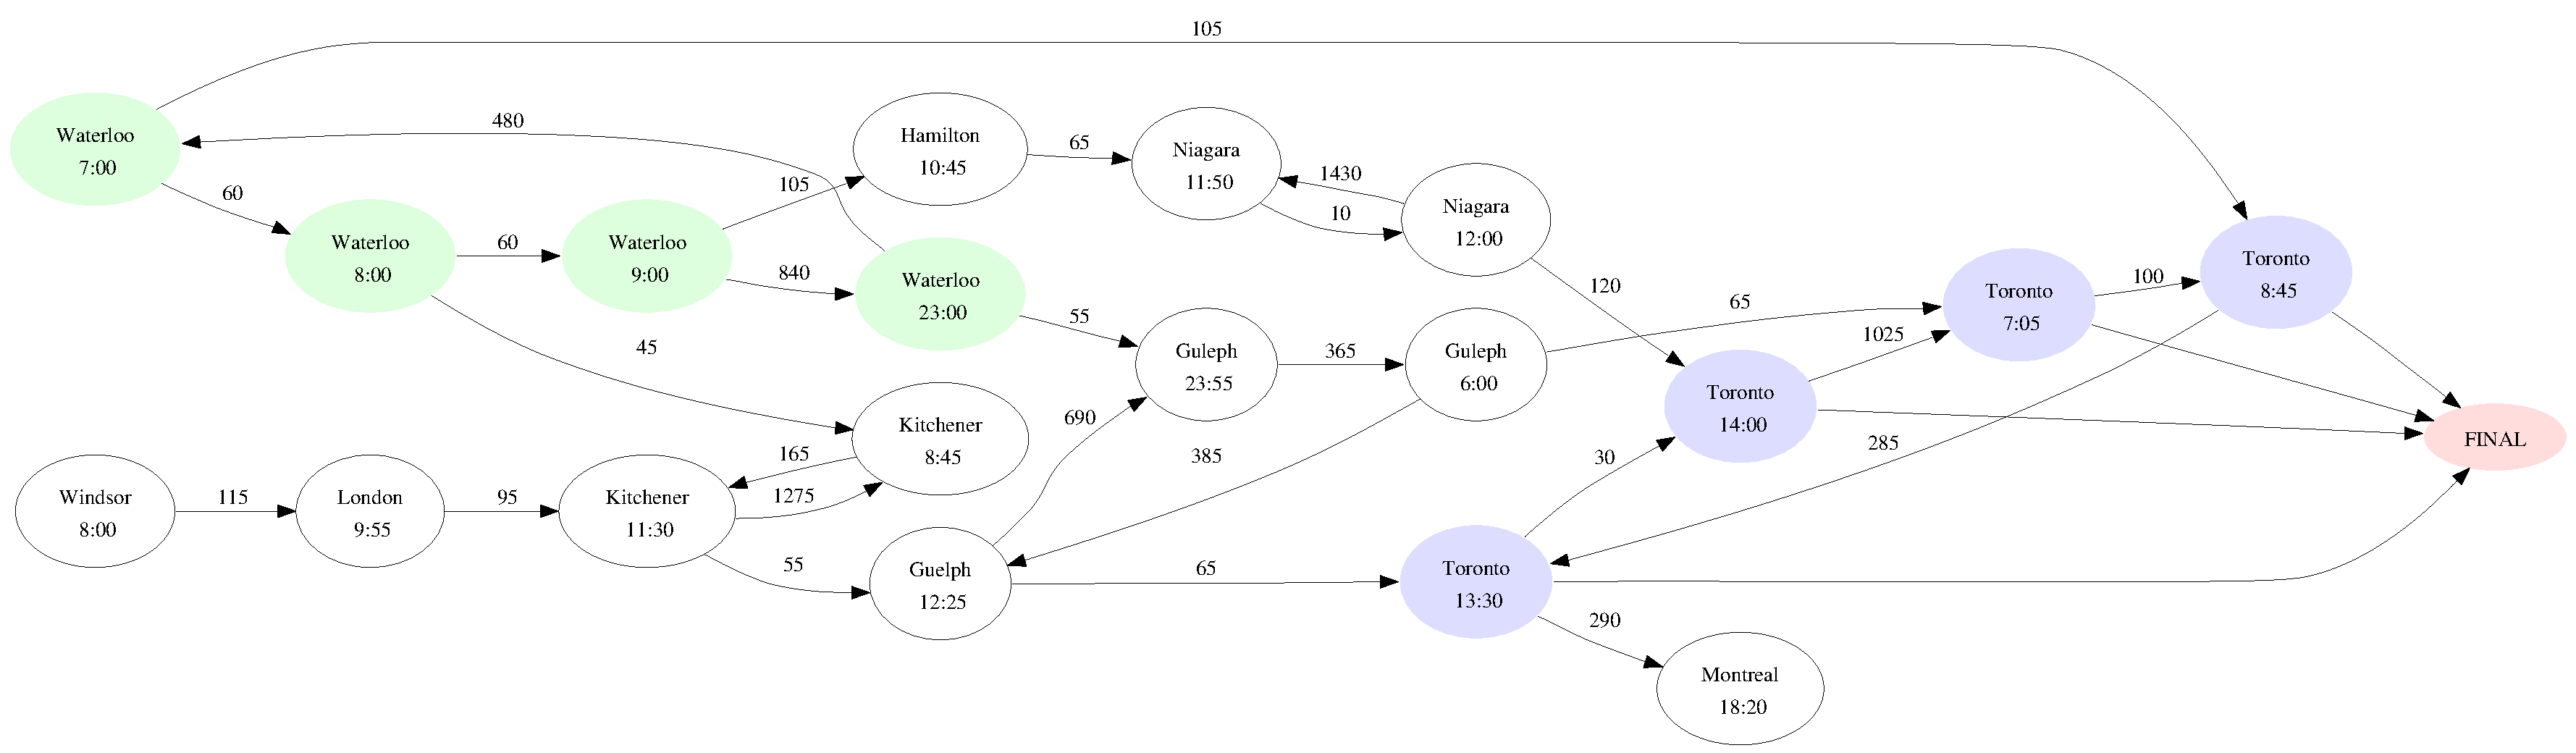
\includegraphics[scale=0.3]{./figuras/grafo.pdf}
\caption{Grafo resultante para la entrada de ejemplo (antes de invertir los ejes)}
\end{figure}

\subsubsection{Determinaci\'on de las conexiones \'optimas}

Una vez obtenidas las duraciones m\'inimas de los caminos que parten de cada
uno de los nodos $(src,h)$, resta s\'olo filtrar de esos caminos aquellos que
cumplen con la condici\'on (A).

Notar que la condici\'on (A) usa la expresi\'on ``llegar m\'as temprano'' en
el sentido que uno le atribuye intuitivamente, y no a la hora absoluta del d�a.
Por ejemplo, salir a las 21:00 y llegar a las 22:00 es llegar m\'as temprano
que salir a las 20:00 y llegar a la 1:00, pese a que $\text{1:00} < \text{22:00}$.
Esto es obvio, pero indica que la implementaci\'on debe comparar las duraciones
totales de los viajes m\'as que las horas de llegada.
Algo similar aplica para la expresi\'on ``salir m\'as tarde''.
%En la resoluci�n del problema consideramos el tiempo como cantidad de minutos.

El siguiente es el algoritmo para elegir las rutas, asumiendo que
las distancias desde cada nodo $v$ hasta el nodo $\textsc{final}$
ya fueron calculadas:

\begin{algorithm}[H]
\begin{algorithmic}
\caption{Determina las conexiones \'optimas}
\PARAMS{$distancia_v$ = duraci\'on m�nima de la conexi\'on desde un nodo $v$ hasta el nodo $\textsc{final}$}
\STATE m�nima hora de llegada $:= \infty$
\FOR{cada nodo $v$ de la forma $(src,h)$}
\STATE hora de llegada $:= h + distancia_{v} + $ 24 hs
\STATE\COMMENT{tiempo del nodo es la cantidad de tiempo hasta que sale el tren (i.e: si el tren sale a las 8, es la cantidad de minutos hasta las 8)}
\STATE m�nima hora de llegada $:= \min($hora de llegada, m�nima hora de llegada$)$
\ENDFOR 
\FOR{cada nodo $v$ de la forma $(src,h)$ (se recorren por hora decreciente)}
%\STATE hora de salida $:= h$
\STATE hora de llegada $:= h + distancia_{v}$
\IF{hora de llegada $<$ m�nima hora de llegada}
\STATE m�nima hora de llegada $:=$ hora de llegada
\STATE reportar la conexi\'on que sale a la hora $h$ y tarda $distancia_{v}$ en llegar
\ENDIF
\ENDFOR
\end{algorithmic}
\end{algorithm}

El primer {\bf for} inicializa el valor de la variable ``m\'inima hora de llegada''.
Para esto se busca, entre todos los nodos $(src,h)$, el que minimiza $h + distancia_{(src,h)} + \text{24 hs}$.
Este valor $H$ representa la hora m\'as temprana a la que se puede llegar a destino partiendo al
d\'ia siguiente, y se usa como cota superior para descartar algunas de las conexiones
que no son \'optimas.
Es decir, si $distancia_{(src,h)} \geq H$, la conexi\'on m\'as corta que empieza
en la estaci\'on de origen tomando el tren de la hora $h$ llega a lo sumo tan temprano
como alguna otra conexi\'on posterior, y por lo tanto no es \'optima.

Notar que alcanza con usar como cota superior la hora de llegada de
la conexi\'on m\'as corta que empieza en el {\em segundo} d\'ia
(y no es necesario mirar m\'as d\'ias hacia adelante) porque
la conexi\'on m\'as corta que empieza en el cualquier d\'ia
posterior al segundo llega despu\'es de $H$.

En el segundo {\bf for}, se tiene como invariante que la variable ``m\'inima hora de llegada''
es la m\'inima hora a la que se puede llegar con una conexi\'on que sale en
una hora posterior a $h$. Inicialmente esto es cierto porque, como ya se justific\'o,
``m\'inima hora de llegada'' se inicializa en $H$. El invariante se mantiene porque
los nodos se recorren por hora decreciente. En cada paso, si la hora a la que se
llega con una conexi\'on que empieza desde el nodo $v$ es menor que la m\'inima
hora a la que se puede llegar saliendo despu\'es de la hora $h$, esto quiere
decir que dicha conexi\'on cumple con la condici\'on (A). Adem\'as, es \'optima
porque tambi\'en cumpl\'ia con la condici\'on (B).

\subsubsection{Detalles de implementaci\'on y complejidad}

Todas las horas se representan en minutos. El grafo se representa con listas
de adyacencia. Cada nodo se identifica mediante un par $\langle id, hora \rangle$,
donde $id$ es un entero que representa una estaci\'on. Las listas de adyacencia se guardan
en un diccionario de nodo a lista de vecinos, cada uno con el peso del eje
correspondiente.

Llamamos $N$ a la cantidad de estaciones y $M$ a la cantidad de ejes
del grafo asociado al problema. Notar que $N \in O(M)$ porque no puede
haber nodos aislados, ya que si una estaci\'on
ocurre en la entrada, debe figurar en al menos una ruta. Adem\'as,
$M$ es lineal en el tama\~no de la entrada, porque
los ejes que representan el camino de un tren deben estar
expl\'icitos en la entrada, mientras la cantidad de ejes que
conectan nodos de la misma estaci\'on es (por la manera en la
que se construye el grafo) a lo sumo igual a la cantidad total
de nodos de la estaci\'on.
% Para construir el grafo, la informaci\'on de las estaciones
%se guarda en un diccionario que dado el nombre de la estaci\'on devuelve su
%id y el conjunto de horas a las que un tren pasa por dicha estaci\'on.

La implementaci\'on del algoritmo de Dijkstra usa una cola de prioridad
representada mediante un conjunto de tuplas $\langle distancia, nodo \rangle$,
por lo que la complejidad del algoritmo es $O(M \log N)$. El costo del
algoritmo que determina las conexiones \'optimas es $O(N \log N)$.
Previo a resolver el problema, el costo de procesar la entrada es el siguiente: 
\begin{itemize}
\item Primero se asigna un id a cada estaci\'on, y se construye un 
diccionario que permite ver, dada una estaci\'on (\texttt{string}), qu\'e
id tiene y a qu� horas hay trenes que llegan o salen. El costo de
esto es $O(N \log N)$ asumiendo, de acuerdo con el enunciado del
problema, que los nombres de las estaciones tienen un largo m\'aximo fijo
(y razonablemente chico).
\item Despu\'es se construyen las listas de adyacencia.
Esto toma $O(M \log N + N \log N)$. El segundo t�rmino proviene del costo de agregar 
los ejes entre nodos de la misma estaci�n. Esto se puede hacer en $O(N \log N)$ iterando las
claves del diccionario que guarda los ids y las horas de cada estaci\'on.
\end{itemize}

Finalmente la complejidad es $O(N \log N + M \log N) \subseteq O(M \log N)$.

\subsection{Implementaci�n}
\noindent
\ttfamily
\shorthandoff{"}\\
\hlstd{}\hlline{\ 1\ }\hldir{\#include\ $<$iostream$>$}\\
\hlline{\ 2\ }\hlstd{}\hldir{\#include\ $<$string$>$}\\
\hlline{\ 3\ }\hlstd{}\hldir{\#include\ $<$map$>$}\\
\hlline{\ 4\ }\hlstd{}\hldir{\#include\ $<$set$>$}\\
\hlline{\ 5\ }\hlstd{}\hldir{\#include\ $<$vector$>$}\\
\hlline{\ 6\ }\hlstd{}\hldir{\#include\ $<$list$>$}\\
\hlline{\ 7\ }\hlstd{}\hldir{\#include\ $<$cassert$>$}\\
\hlline{\ 8\ }\hlstd{}\hldir{\#include\ $<$cstdlib$>$}\\
\hlline{\ 9\ }\hlstd{}\\
\hlline{10\ }\hlkwa{using\ namespace\ }\hlstd{std}\hlsym{;}\\
\hlline{11\ }\hlstd{}\\
\hlline{12\ }\hldir{\#define\ forsn(i,\ s,\ n)\ for\ (int\ i\ =\ (s);\ i\ $<$\ (n);\ i++)}\\
\hlline{13\ }\hlstd{}\hldir{\#define\ forn(i,\ n)}\hlstd{\ \ }\hldir{forsn\ (i,\ 0,\ n)}\\
\hlline{14\ }\hlstd{}\hldir{\#define\ forall(x,\ s)\ for\ (typeof((s).begin())\ x\ =\ (s).begin();\ x\ !=\ (s).end();\ x++)}\\
\hlline{15\ }\hlstd{}\hldir{\#define\ dforall(x,\ s)\ for\ (typeof((s).rbegin())\ x\ =\ (s).rbegin();\ x\ !=\ (s).rend();\ x++)}\\
\hlline{16\ }\hlstd{}\\
\hlline{17\ }\hlkwc{typedef\ }\hlstd{}\hlkwb{int\ }\hlstd{Id}\hlsym{;\ }\hlstd{}\hlslc{//\ station\ id}\\
\hlline{18\ }\hlstd{}\hlkwc{typedef\ }\hlstd{}\hlkwb{int\ }\hlstd{Time}\hlsym{;}\\
\hlline{19\ }\hlstd{}\hlkwc{typedef\ }\hlstd{pair}\hlsym{$<$}\hlstd{Id}\hlsym{,\ }\hlstd{Time}\hlsym{$>$\ }\hlstd{Nodo}\hlsym{;}\\
\hlline{20\ }\hlstd{}\\
\hlline{21\ }\hlkwb{struct\ }\hlstd{Edge\ }\hlsym{\{}\\
\hlline{22\ }\hlstd{\ Nodo\ dest}\hlsym{;}\\
\hlline{23\ }\hlstd{\ Time\ cost}\hlsym{;}\\
\hlline{24\ }\hlstd{}\hlsym{\};}\\
\hlline{25\ }\hlstd{}\hlkwc{typedef\ }\hlstd{vector}\hlsym{$<$}\hlstd{Edge}\hlsym{$>$\ }\hlstd{Ady}\hlsym{;}\\
\hlline{26\ }\hlstd{}\hlkwc{typedef\ }\hlstd{map}\hlsym{$<$}\hlstd{Nodo}\hlsym{,\ }\hlstd{Ady}\hlsym{$>$\ }\hlstd{Grafo}\hlsym{;}\\
\hlline{27\ }\hlstd{}\\
\hlline{28\ }\hlkwc{typedef\ }\hlstd{map}\hlsym{$<$}\hlstd{string}\hlsym{,\ }\hlstd{pair}\hlsym{$<$}\hlstd{Id}\hlsym{,\ }\hlstd{set}\hlsym{$<$}\hlstd{Time}\hlsym{$>$\ $>$\ $>$\ }\hlstd{Stations}\hlsym{;}\\
\hlline{29\ }\hlstd{}\\
\hlline{30\ }\hlslc{//\ map$<$Nodo,\ Ady$>$::iterator}\\
\hlline{31\ }\hlstd{}\hldir{\#define\ \textunderscore nodo}\hlstd{\ \ }\hldir{first}\\
\hlline{32\ }\hlstd{}\hldir{\#define\ \textunderscore ady}\hlstd{\ \ }\hldir{second}\\
\hlline{33\ }\hlstd{}\\
\hlline{34\ }\hlslc{//\ Stations::iterator}\\
\hlline{35\ }\hlstd{}\hldir{\#define\ \textunderscore info}\hlstd{\ \ }\hldir{second}\\
\hlline{36\ }\hlstd{}\\
\hlline{37\ }\hlslc{//\ pair$<$Id,\ set$<$Time$>$\ $>$}\\
\hlline{38\ }\hlstd{}\hldir{\#define\ \textunderscore id}\hlstd{\ \ }\hldir{first}\\
\hlline{39\ }\hlstd{}\hldir{\#define\ \textunderscore timeset\ second}\\
\hlline{40\ }\hlstd{}\\
\hlline{41\ }\hlslc{//\ Nodo}\\
\hlline{42\ }\hlstd{}\hldir{\#define\ \textunderscore time}\hlstd{\ \ }\hldir{second}\\
\hlline{43\ }\hlstd{}\\
\hlline{44\ }\hldir{\#define\ HOUR\ 60}\\
\hlline{45\ }\hlstd{}\hldir{\#define\ DAY\ (24\ {*}\ HOUR)}\\
\hlline{46\ }\hlstd{\\
\hlline{47\ }Id\ }\hlkwc{inline\ }\hlstd{}\hlkwd{register\textunderscore station}\hlstd{}\hlsym{(}\hlstd{Stations}\hlsym{\&\ }\hlstd{stations}\hlsym{,\ }\hlstd{}\hlkwb{const\ }\hlstd{string}\hlsym{\&\ }\hlstd{station\textunderscore name}\hlsym{,\ }\hlstd{Time\ time}\hlsym{)\ \{}\\
\hlline{48\ }\hlstd{\ Stations}\hlsym{::}\hlstd{iterator\ }\hlkwd{it}\hlstd{}\hlsym{(}\hlstd{stations}\hlsym{.}\hlstd{}\hlkwd{find}\hlstd{}\hlsym{(}\hlstd{station\textunderscore name}\hlsym{));}\\
\hlline{49\ }\hlstd{\ }\hlkwa{if\ }\hlstd{}\hlsym{(}\hlstd{it\ }\hlsym{==\ }\hlstd{stations}\hlsym{.}\hlstd{}\hlkwd{end}\hlstd{}\hlsym{())\ \{}\\
\hlline{50\ }\hlstd{}\hlstd{\ \ }\hlstd{}\hlslc{//\ create}\\
\hlline{51\ }\hlstd{}\hlstd{\ \ }\hlstd{}\hlkwb{const\ }\hlstd{Id\ a\ }\hlsym{=\ }\hlstd{stations}\hlsym{.}\hlstd{}\hlkwd{size}\hlstd{}\hlsym{();}\\
\hlline{52\ }\hlstd{}\hlstd{\ \ }\hlstd{set}\hlsym{$<$}\hlstd{Time}\hlsym{$>$\ }\hlstd{s}\hlsym{;}\\
\hlline{53\ }\hlstd{}\hlstd{\ \ }\hlstd{s}\hlsym{.}\hlstd{}\hlkwd{insert}\hlstd{}\hlsym{(}\hlstd{time}\hlsym{);}\\
\hlline{54\ }\hlstd{}\hlstd{\ \ }\hlstd{stations}\hlsym{{[}}\hlstd{station\textunderscore name}\hlsym{{]}\ =\ }\hlstd{pair}\hlsym{$<$}\hlstd{Id}\hlsym{,\ }\hlstd{set}\hlsym{$<$}\hlstd{Time}\hlsym{$>$\ $>$(}\hlstd{a}\hlsym{,\ }\hlstd{s}\hlsym{);}\\
\hlline{55\ }\hlstd{}\hlstd{\ \ }\hlstd{}\hlkwa{return\ }\hlstd{a}\hlsym{;}\\
\hlline{56\ }\hlstd{\ }\hlsym{\}\ }\hlstd{}\hlkwa{else\ }\hlstd{}\hlsym{\{}\\
\hlline{57\ }\hlstd{}\hlstd{\ \ }\hlstd{pair}\hlsym{$<$}\hlstd{Id}\hlsym{,}\hlstd{set}\hlsym{$<$}\hlstd{Time}\hlsym{$>$\ $>$\&\ }\hlstd{t\ }\hlsym{=\ }\hlstd{stations}\hlsym{{[}}\hlstd{station\textunderscore name}\hlsym{{]};}\\
\hlline{58\ }\hlstd{}\hlstd{\ \ }\hlstd{t}\hlsym{.}\hlstd{\textunderscore timeset}\hlsym{.}\hlstd{}\hlkwd{insert}\hlstd{}\hlsym{(}\hlstd{time}\hlsym{);}\\
\hlline{59\ }\hlstd{}\hlstd{\ \ }\hlstd{}\hlkwa{return\ }\hlstd{t}\hlsym{.}\hlstd{\textunderscore id}\hlsym{;}\\
\hlline{60\ }\hlstd{\ }\hlsym{\}}\\
\hlline{61\ }\hlstd{}\hlsym{\}}\\
\hlline{62\ }\hlstd{}\\
\hlline{63\ }\hlkwc{inline\ }\hlstd{}\hlkwb{int\ }\hlstd{}\hlkwd{time\textunderscore in\textunderscore minutes}\hlstd{}\hlsym{(}\hlstd{string}\hlsym{\&\ }\hlstd{s}\hlsym{)\ \{}\\
\hlline{64\ }\hlstd{\ }\hlslc{//\ h:mm\ hh:mm\ hhh:mm\ ...}\\
\hlline{65\ }\hlstd{\ }\hlkwb{const\ int\ }\hlstd{l\ }\hlsym{=\ }\hlstd{s}\hlsym{.}\hlstd{}\hlkwd{size}\hlstd{}\hlsym{();}\\
\hlline{66\ }\hlstd{\ }\hlkwd{assert}\hlstd{}\hlsym{(}\hlstd{s}\hlsym{{[}}\hlstd{l\ }\hlsym{{-}\ }\hlstd{}\hlnum{3}\hlstd{}\hlsym{{]}\ ==\ }\hlstd{}\hlstr{`:`}\hlstd{}\hlsym{);}\\
\hlline{67\ }\hlstd{\ }\hlkwa{return\ }\hlstd{}\hlkwd{atoi}\hlstd{}\hlsym{(}\hlstd{s}\hlsym{.}\hlstd{}\hlkwd{substr}\hlstd{}\hlsym{(}\hlstd{}\hlnum{0}\hlstd{}\hlsym{,\ }\hlstd{l\ }\hlsym{{-}\ }\hlstd{}\hlnum{3}\hlstd{}\hlsym{).}\hlstd{}\hlkwd{c\textunderscore str}\hlstd{}\hlsym{())\ {*}\ }\hlstd{HOUR\ }\hlsym{+\ }\hlstd{}\hlkwd{atoi}\hlstd{}\hlsym{(}\hlstd{s}\hlsym{.}\hlstd{}\hlkwd{substr}\hlstd{}\hlsym{(}\hlstd{l\ }\hlsym{{-}\ }\hlstd{}\hlnum{2}\hlstd{}\hlsym{,\ }\hlstd{}\hlnum{2}\hlstd{}\hlsym{).}\hlstd{}\hlkwd{c\textunderscore str}\hlstd{}\hlsym{());}\\
\hlline{68\ }\hlstd{}\hlsym{\}}\\
\hlline{69\ }\hlstd{}\\
\hlline{70\ }\hlkwb{void\ }\hlstd{}\hlkwd{print\textunderscore graph}\hlstd{}\hlsym{(}\hlstd{Grafo}\hlsym{\&\ }\hlstd{g}\hlsym{)\ \{}\\
\hlline{71\ }\hlstd{\ }\hlkwd{forall\ }\hlstd{}\hlsym{(}\hlstd{x}\hlsym{,\ }\hlstd{g}\hlsym{)\ \{}\\
\hlline{72\ }\hlstd{}\hlstd{\ \ }\hlstd{cout\ }\hlsym{$<$$<$\ }\hlstd{}\hlstr{"Hasta:\ "}\hlstd{\ }\hlsym{$<$$<$\ }\hlstd{x}\hlsym{{-}$>$}\hlstd{\textunderscore nodo}\hlsym{.}\hlstd{\textunderscore id\ }\hlsym{$<$$<$\ }\hlstd{}\hlstr{"\ a\ las\ "}\hlstd{\ }\hlsym{$<$$<$\ (}\hlstd{x}\hlsym{{-}$>$}\hlstd{\textunderscore nodo}\hlsym{.}\hlstd{\textunderscore time\ }\hlsym{/\ }\hlstd{}\hlnum{60}\hlstd{}\hlsym{)\ $<$$<$\ }\hlstd{}\hlstr{":"}\hlstd{\ }\hlsym{$<$$<$\ (}\hlstd{x}\hlsym{{-}$>$}\hlstd{\textunderscore nodo}\hlsym{.}\hlstd{\textunderscore time\ \Righttorque\\
\hlline{73\ }}\hlstd{\ \ \ \ \ \ \ \ \ \ \ \ \ \ \ \ \ \ \ \ \ \ \ \ \ \ \ \ \ \ \ \ \ \ \ \ \ \ \ \ \ \ \ \ \ \ \ \ \ \ \ \ \ }\hlstd{}\hlsym{\%\ }\hlstd{}\hlnum{60}\hlstd{}\hlsym{)\ $<$$<$\ }\hlstd{endl}\hlsym{;}\\
\hlline{74\ }\hlstd{}\hlstd{\ \ }\hlstd{}\hlkwd{forall\ }\hlstd{}\hlsym{(}\hlstd{y}\hlsym{,\ }\hlstd{x}\hlsym{{-}$>$}\hlstd{\textunderscore ady}\hlsym{)\ \{}\\
\hlline{75\ }\hlstd{}\hlstd{\ \ \ }\hlstd{cout\ }\hlsym{$<$$<$\ }\hlstd{}\hlstr{"}\hlstd{\ \ \ \ }\hlstr{desde\ "}\hlstd{\ }\hlsym{$<$$<$\ }\hlstd{y}\hlsym{{-}$>$}\hlstd{dest}\hlsym{.}\hlstd{\textunderscore id\\
\hlline{76\ }}\hlstd{\ \ \ \ }\hlstd{}\hlsym{$<$$<$\ }\hlstd{}\hlstr{"\ a\ las\ "}\hlstd{\ }\hlsym{$<$$<$\ (}\hlstd{y}\hlsym{{-}$>$}\hlstd{dest}\hlsym{.}\hlstd{\textunderscore time\ }\hlsym{/\ }\hlstd{}\hlnum{60}\hlstd{}\hlsym{)\ $<$$<$\ }\hlstd{}\hlstr{":"}\hlstd{\ }\hlsym{$<$$<$\ (}\hlstd{y}\hlsym{{-}$>$}\hlstd{dest}\hlsym{.}\hlstd{\textunderscore time\ }\hlsym{\%\ }\hlstd{}\hlnum{60}\hlstd{}\hlsym{)}\\
\hlline{77\ }\hlstd{}\hlstd{\ \ \ \ }\hlstd{}\hlsym{$<$$<$\ }\hlstd{}\hlstr{"\ costo:\ "}\hlstd{\ }\hlsym{$<$$<$\ (}\hlstd{y}\hlsym{{-}$>$}\hlstd{cost\ }\hlsym{/\ }\hlstd{}\hlnum{60}\hlstd{}\hlsym{)\ $<$$<$\ }\hlstd{}\hlstr{":"}\hlstd{\ }\hlsym{$<$$<$\ (}\hlstd{y}\hlsym{{-}$>$}\hlstd{cost\ }\hlsym{\%\ }\hlstd{}\hlnum{60}\hlstd{}\hlsym{)\ $<$$<$\ }\hlstd{endl}\hlsym{;}\\
\hlline{78\ }\hlstd{}\hlstd{\ \ }\hlstd{}\hlsym{\}}\\
\hlline{79\ }\hlstd{\ }\hlsym{\}}\\
\hlline{80\ }\hlstd{}\hlsym{\}}\\
\hlline{81\ }\hlstd{}\\
\hlline{82\ }\hldir{\#define\ INF\ 0x7fffffff}\\
\hlline{83\ }\hlstd{}\\
\hlline{84\ }\hlkwc{inline\ }\hlstd{}\hlkwb{void\ }\hlstd{}\hlkwd{dijkstra}\hlstd{}\hlsym{(}\hlstd{Stations}\hlsym{\&\ }\hlstd{stations}\hlsym{,\ }\hlstd{Grafo}\hlsym{\&\ }\hlstd{graph}\hlsym{,\ }\hlstd{}\hlkwb{const\ }\hlstd{string}\hlsym{\&\ }\hlstd{origen}\hlsym{,\ }\hlstd{}\hlkwb{const\ }\hlstd{string}\hlsym{\&\ }\hlstd{destino}\hlsym{)\ \{}\\
\hlline{85\ }\hlstd{\ }\hlkwb{const\ }\hlstd{Id\ id\textunderscore origen\ }\hlsym{=\ }\hlstd{stations}\hlsym{{[}}\hlstd{origen}\hlsym{{]}.}\hlstd{\textunderscore id}\hlsym{;}\\
\hlline{86\ }\hlstd{\ }\hlkwb{const\ }\hlstd{Id\ id\textunderscore destino\ }\hlsym{=\ }\hlstd{stations}\hlsym{{[}}\hlstd{destino}\hlsym{{]}.}\hlstd{\textunderscore id}\hlsym{;}\\
\hlline{87\ }\hlstd{\\
\hlline{88\ }\ set}\hlsym{$<$}\hlstd{pair}\hlsym{$<$}\hlstd{Time}\hlsym{,\ }\hlstd{Nodo}\hlsym{$>$\ $>$\ }\hlstd{cola}\hlsym{;}\\
\hlline{89\ }\hlstd{\ map}\hlsym{$<$}\hlstd{Nodo}\hlsym{,\ }\hlstd{Time}\hlsym{$>$\ }\hlstd{distancia}\hlsym{;}\\
\hlline{90\ }\hlstd{\\
\hlline{91\ }\ }\hlslc{//\ inicializar\ distancias}\\
\hlline{92\ }\hlstd{\ }\hlkwd{forall\ }\hlstd{}\hlsym{(}\hlstd{st}\hlsym{,\ }\hlstd{stations}\hlsym{)\ \{}\\
\hlline{93\ }\hlstd{}\hlstd{\ \ }\hlstd{Id\ station\textunderscore id\ }\hlsym{=\ }\hlstd{st}\hlsym{{-}$>$}\hlstd{\textunderscore info}\hlsym{.}\hlstd{\textunderscore id}\hlsym{;}\\
\hlline{94\ }\hlstd{}\hlstd{\ \ }\hlstd{}\hlkwd{forall\ }\hlstd{}\hlsym{(}\hlstd{t}\hlsym{,\ }\hlstd{st}\hlsym{{-}$>$}\hlstd{\textunderscore info}\hlsym{.}\hlstd{\textunderscore timeset}\hlsym{)\ \{}\\
\hlline{95\ }\hlstd{}\hlstd{\ \ \ }\hlstd{Nodo\ }\hlkwd{v}\hlstd{}\hlsym{(}\hlstd{station\textunderscore id}\hlsym{,\ {*}}\hlstd{t}\hlsym{);}\\
\hlline{96\ }\hlstd{}\hlstd{\ \ \ }\hlstd{}\hlkwa{if\ }\hlstd{}\hlsym{(}\hlstd{station\textunderscore id\ }\hlsym{==\ }\hlstd{id\textunderscore destino}\hlsym{)\ \{}\\
\hlline{97\ }\hlstd{}\hlstd{\ \ \ \ }\hlstd{cola}\hlsym{.}\hlstd{}\hlkwd{insert}\hlstd{}\hlsym{(}\hlstd{pair}\hlsym{$<$}\hlstd{Time}\hlsym{,}\hlstd{Nodo}\hlsym{$>$(}\hlstd{}\hlnum{0}\hlstd{}\hlsym{,\ }\hlstd{v}\hlsym{));}\\
\hlline{98\ }\hlstd{}\hlstd{\ \ \ \ }\hlstd{distancia}\hlsym{{[}}\hlstd{v}\hlsym{{]}\ =\ }\hlstd{}\hlnum{0}\hlstd{}\hlsym{;}\\
\hlline{99\ }\hlstd{}\hlstd{\ \ \ }\hlstd{}\hlsym{\}\ }\hlstd{}\hlkwa{else\ }\hlstd{}\hlsym{\{}\\
\hlline{100\ }\hlstd{}\hlstd{\ \ \ \ }\hlstd{distancia}\hlsym{{[}}\hlstd{v}\hlsym{{]}\ =\ }\hlstd{INF}\hlsym{;}\\
\hlline{101\ }\hlstd{}\hlstd{\ \ \ }\hlstd{}\hlsym{\}}\\
\hlline{102\ }\hlstd{}\hlstd{\ \ }\hlstd{}\hlsym{\}}\\
\hlline{103\ }\hlstd{\ }\hlsym{\}}\\
\hlline{104\ }\hlstd{\ }\hlkwa{while\ }\hlstd{}\hlsym{(!}\hlstd{cola}\hlsym{.}\hlstd{}\hlkwd{empty}\hlstd{}\hlsym{())\ \{}\\
\hlline{105\ }\hlstd{}\hlstd{\ \ }\hlstd{}\hlslc{//\ buscar\ el\ minimo}\\
\hlline{106\ }\hlstd{}\hlstd{\ \ }\hlstd{Time\ min\textunderscore dist\ }\hlsym{=\ }\hlstd{cola}\hlsym{.}\hlstd{}\hlkwd{begin}\hlstd{}\hlsym{(){-}$>$}\hlstd{first}\hlsym{;}\\
\hlline{107\ }\hlstd{\\
\hlline{108\ }}\hlstd{\ \ }\hlstd{}\hlslc{//\ borrarlo\ de\ la\ cola}\\
\hlline{109\ }\hlstd{}\hlstd{\ \ }\hlstd{Nodo\ min\textunderscore node\ }\hlsym{=\ }\hlstd{cola}\hlsym{.}\hlstd{}\hlkwd{begin}\hlstd{}\hlsym{(){-}$>$}\hlstd{second}\hlsym{;}\\
\hlline{110\ }\hlstd{}\hlstd{\ \ }\hlstd{cola}\hlsym{.}\hlstd{}\hlkwd{erase}\hlstd{}\hlsym{(}\hlstd{cola}\hlsym{.}\hlstd{}\hlkwd{begin}\hlstd{}\hlsym{());}\\
\hlline{111\ }\hlstd{\\
\hlline{112\ }}\hlstd{\ \ }\hlstd{}\hlslc{//\ procesar\ min\textunderscore node}\\
\hlline{113\ }\hlstd{}\hlstd{\ \ }\hlstd{}\hlkwd{forall\ }\hlstd{}\hlsym{(}\hlstd{eje}\hlsym{,\ }\hlstd{graph}\hlsym{{[}}\hlstd{min\textunderscore node}\hlsym{{]})\ \{}\\
\hlline{114\ }\hlstd{}\hlstd{\ \ \ }\hlstd{}\hlkwb{const\ }\hlstd{Time\ dist\textunderscore nueva\ }\hlsym{=\ }\hlstd{min\textunderscore dist\ }\hlsym{+\ }\hlstd{eje}\hlsym{{-}$>$}\hlstd{cost}\hlsym{;}\\
\hlline{115\ }\hlstd{}\hlstd{\ \ \ \ \ \ \ \ \ \ \ \ \ \ \ \ \ \ \ \ \ \ \ \ }\hlstd{}\hlkwb{const\ }\hlstd{Time\ dist\textunderscore actual\ }\hlsym{=\ }\hlstd{distancia}\hlsym{{[}}\hlstd{eje}\hlsym{{-}$>$}\hlstd{dest}\hlsym{{]};}\\
\hlline{116\ }\hlstd{}\hlstd{\ \ \ }\hlstd{}\hlkwa{if\ }\hlstd{}\hlsym{(}\hlstd{dist\textunderscore nueva\ }\hlsym{$<$\ }\hlstd{dist\textunderscore actual}\hlsym{)\ \{}\\
\hlline{117\ }\hlstd{}\hlstd{\ \ \ \ }\hlstd{}\hlkwa{if\ }\hlstd{}\hlsym{(}\hlstd{dist\textunderscore actual\ }\hlsym{!=\ }\hlstd{INF}\hlsym{)\ \{}\\
\hlline{118\ }\hlstd{}\hlstd{\ \ \ \ \ }\hlstd{cola}\hlsym{.}\hlstd{}\hlkwd{erase}\hlstd{}\hlsym{(}\hlstd{cola}\hlsym{.}\hlstd{}\hlkwd{find}\hlstd{}\hlsym{(}\hlstd{pair}\hlsym{$<$}\hlstd{Time}\hlsym{,}\hlstd{Nodo}\hlsym{$>$(}\hlstd{dist\textunderscore actual}\hlsym{,\ }\hlstd{eje}\hlsym{{-}$>$}\hlstd{dest}\hlsym{)));}\\
\hlline{119\ }\hlstd{}\hlstd{\ \ \ \ }\hlstd{}\hlsym{\}}\\
\hlline{120\ }\hlstd{}\hlstd{\ \ \ \ }\hlstd{distancia}\hlsym{{[}}\hlstd{eje}\hlsym{{-}$>$}\hlstd{dest}\hlsym{{]}\ =\ }\hlstd{dist\textunderscore nueva}\hlsym{;}\\
\hlline{121\ }\hlstd{}\hlstd{\ \ \ \ }\hlstd{cola}\hlsym{.}\hlstd{}\hlkwd{insert}\hlstd{}\hlsym{(}\hlstd{pair}\hlsym{$<$}\hlstd{Time}\hlsym{,}\hlstd{Nodo}\hlsym{$>$(}\hlstd{dist\textunderscore nueva}\hlsym{,\ }\hlstd{eje}\hlsym{{-}$>$}\hlstd{dest}\hlsym{));}\\
\hlline{122\ }\hlstd{}\hlstd{\ \ \ }\hlstd{}\hlsym{\}}\\
\hlline{123\ }\hlstd{}\hlstd{\ \ }\hlstd{}\hlsym{\}}\\
\hlline{124\ }\hlstd{\ }\hlsym{\}}\\
\hlline{125\ }\hlstd{\\
\hlline{126\ }\ list}\hlsym{$<$}\hlstd{pair}\hlsym{$<$}\hlstd{Time}\hlsym{,\ }\hlstd{Time}\hlsym{$>$\ $>$\ }\hlstd{salida}\hlsym{;}\\
\hlline{127\ }\hlstd{\ Time\ min\textunderscore hora\textunderscore llega\ }\hlsym{=\ }\hlstd{INF}\hlsym{;}\\
\hlline{128\ }\hlstd{\ }\hlkwd{forall\ }\hlstd{}\hlsym{(}\hlstd{t}\hlsym{,\ }\hlstd{stations}\hlsym{{[}}\hlstd{origen}\hlsym{{]}.}\hlstd{\textunderscore timeset}\hlsym{)\ \{}\\
\hlline{129\ }\hlstd{}\hlstd{\ \ }\hlstd{Nodo\ }\hlkwd{v}\hlstd{}\hlsym{(}\hlstd{id\textunderscore origen}\hlsym{,\ {*}}\hlstd{t}\hlsym{);}\\
\hlline{130\ }\hlstd{}\hlstd{\ \ }\hlstd{}\hlkwb{const\ }\hlstd{Time\ hora\textunderscore llega\ }\hlsym{=\ {*}}\hlstd{t\ }\hlsym{+\ }\hlstd{distancia}\hlsym{{[}}\hlstd{v}\hlsym{{]}\ +\ }\hlstd{DAY}\hlsym{;}\\
\hlline{131\ }\hlstd{}\hlstd{\ \ }\hlstd{min\textunderscore hora\textunderscore llega\ }\hlsym{=\ }\hlstd{}\hlkwd{min}\hlstd{}\hlsym{(}\hlstd{min\textunderscore hora\textunderscore llega}\hlsym{,\ }\hlstd{hora\textunderscore llega}\hlsym{);}\\
\hlline{132\ }\hlstd{\ }\hlsym{\}}\\
\hlline{133\ }\hlstd{\ }\hlkwd{dforall\ }\hlstd{}\hlsym{(}\hlstd{t}\hlsym{,\ }\hlstd{stations}\hlsym{{[}}\hlstd{origen}\hlsym{{]}.}\hlstd{\textunderscore timeset}\hlsym{)\ \{}\\
\hlline{134\ }\hlstd{}\hlstd{\ \ }\hlstd{Nodo\ }\hlkwd{v}\hlstd{}\hlsym{(}\hlstd{id\textunderscore origen}\hlsym{,\ {*}}\hlstd{t}\hlsym{);}\\
\hlline{135\ }\hlstd{}\hlstd{\ \ }\hlstd{}\hlkwb{const\ }\hlstd{Time\ hora\textunderscore sale\ }\hlsym{=\ {*}}\hlstd{t}\hlsym{;}\\
\hlline{136\ }\hlstd{}\hlstd{\ \ }\hlstd{}\hlkwb{const\ }\hlstd{Time\ hora\textunderscore llega\ }\hlsym{=\ {*}}\hlstd{t\ }\hlsym{+\ }\hlstd{distancia}\hlsym{{[}}\hlstd{v}\hlsym{{]};}\\
\hlline{137\ }\hlstd{}\hlstd{\ \ }\hlstd{}\hlkwa{if\ }\hlstd{}\hlsym{(}\hlstd{hora\textunderscore llega\ }\hlsym{$>$=\ }\hlstd{min\textunderscore hora\textunderscore llega}\hlsym{)\ }\hlstd{}\hlkwa{continue}\hlstd{}\hlsym{;}\\
\hlline{138\ }\hlstd{}\hlstd{\ \ }\hlstd{min\textunderscore hora\textunderscore llega\ }\hlsym{=\ }\hlstd{hora\textunderscore llega}\hlsym{;}\\
\hlline{139\ }\hlstd{}\hlstd{\ \ }\hlstd{salida}\hlsym{.}\hlstd{}\hlkwd{push\textunderscore front}\hlstd{}\hlsym{(}\hlstd{pair}\hlsym{$<$}\hlstd{Time}\hlsym{,\ }\hlstd{Time}\hlsym{$>$(}\hlstd{hora\textunderscore sale}\hlsym{,\ }\hlstd{distancia}\hlsym{{[}}\hlstd{v}\hlsym{{]}));}\\
\hlline{140\ }\hlstd{\ }\hlsym{\}}\\
\hlline{141\ }\hlstd{\ }\hlkwd{forall\ }\hlstd{}\hlsym{(}\hlstd{res}\hlsym{,\ }\hlstd{salida}\hlsym{)\ \{}\\
\hlline{142\ }\hlstd{}\hlstd{\ \ }\hlstd{}\hlkwd{printf}\hlstd{}\hlsym{(}\hlstd{}\hlstr{"\%.2i:\%.2i\ "}\hlstd{}\hlsym{,\ }\hlstd{res}\hlsym{{-}$>$}\hlstd{first\ }\hlsym{/\ }\hlstd{}\hlnum{60}\hlstd{}\hlsym{,\ }\hlstd{res}\hlsym{{-}$>$}\hlstd{first\ }\hlsym{\%\ }\hlstd{}\hlnum{60}\hlstd{}\hlsym{);}\\
\hlline{143\ }\hlstd{}\hlstd{\ \ }\hlstd{}\hlkwd{printf}\hlstd{}\hlsym{(}\hlstd{}\hlstr{"\%i:\%.2i}\hlesc{$\backslash$n}\hlstr{"}\hlstd{}\hlsym{,\ }\hlstd{res}\hlsym{{-}$>$}\hlstd{second\ }\hlsym{/\ }\hlstd{}\hlnum{60}\hlstd{}\hlsym{,\ }\hlstd{res}\hlsym{{-}$>$}\hlstd{second\ }\hlsym{\%\ }\hlstd{}\hlnum{60}\hlstd{}\hlsym{);}\\
\hlline{144\ }\hlstd{\ }\hlsym{\}}\\
\hlline{145\ }\hlstd{}\hlsym{\}}\\
\hlline{146\ }\hlstd{}\\
\hlline{147\ }\hldir{\#define\ add\textunderscore edge(g,\ v1,\ v2,\ c)\ ((g){[}(v1){]}.push\textunderscore back((Edge)\{dest:\ (v2),\ cost:\ (c)\}))}\\
\hlline{148\ }\hlstd{}\hlkwb{int\ }\hlstd{}\hlkwd{main}\hlstd{}\hlsym{()\ \{}\\
\hlline{149\ }\hlstd{\ }\hlkwb{int\ }\hlstd{ncases}\hlsym{;}\\
\hlline{150\ }\hlstd{\ cin\ }\hlsym{$>$$>$\ }\hlstd{ncases}\hlsym{;}\\
\hlline{151\ }\hlstd{\\
\hlline{152\ }\ }\hlkwd{forn\ }\hlstd{}\hlsym{(}\hlstd{c}\hlsym{,\ }\hlstd{ncases}\hlsym{)\ \{}\\
\hlline{153\ }\hlstd{}\hlstd{\ \ }\hlstd{Stations\ stations}\hlsym{;}\\
\hlline{154\ }\hlstd{}\hlstd{\ \ }\hlstd{Grafo\ graph}\hlsym{;}\\
\hlline{155\ }\hlstd{\\
\hlline{156\ }}\hlstd{\ \ }\hlstd{}\hlkwb{int\ }\hlstd{num\textunderscore trains}\hlsym{;}\\
\hlline{157\ }\hlstd{}\hlstd{\ \ }\hlstd{cin\ }\hlsym{$>$$>$\ }\hlstd{num\textunderscore trains}\hlsym{;}\\
\hlline{158\ }\hlstd{\\
\hlline{159\ }}\hlstd{\ \ }\hlstd{}\hlslc{//\ read\ trains\ and\ stations}\\
\hlline{160\ }\hlstd{}\hlstd{\ \ }\hlstd{}\hlkwd{forn\ }\hlstd{}\hlsym{(}\hlstd{t}\hlsym{,\ }\hlstd{num\textunderscore trains}\hlsym{)\ \{}\\
\hlline{161\ }\hlstd{}\hlstd{\ \ \ }\hlstd{}\hlkwb{int\ }\hlstd{num\textunderscore stations}\hlsym{;}\\
\hlline{162\ }\hlstd{}\hlstd{\ \ \ }\hlstd{cin\ }\hlsym{$>$$>$\ }\hlstd{num\textunderscore stations}\hlsym{;}\\
\hlline{163\ }\hlstd{\\
\hlline{164\ }}\hlstd{\ \ \ }\hlstd{Nodo\ prev}\hlsym{;}\\
\hlline{165\ }\hlstd{}\hlstd{\ \ \ }\hlstd{}\hlkwb{int\ }\hlstd{time\ }\hlsym{=\ }\hlstd{}\hlnum{0}\hlstd{}\hlsym{;}\\
\hlline{166\ }\hlstd{}\hlstd{\ \ \ }\hlstd{}\hlkwd{forn\ }\hlstd{}\hlsym{(}\hlstd{s}\hlsym{,\ }\hlstd{num\textunderscore stations}\hlsym{)\ \{}\\
\hlline{167\ }\hlstd{}\hlstd{\ \ \ \ }\hlstd{string\ time\textunderscore str}\hlsym{,\ }\hlstd{station\textunderscore name}\hlsym{;}\\
\hlline{168\ }\hlstd{}\hlstd{\ \ \ \ }\hlstd{cin\ }\hlsym{$>$$>$\ }\hlstd{time\textunderscore str\ }\hlsym{$>$$>$\ }\hlstd{station\textunderscore name}\hlsym{;}\\
\hlline{169\ }\hlstd{\\
\hlline{170\ }}\hlstd{\ \ \ \ }\hlstd{}\hlkwb{const\ }\hlstd{Time\ cost\ }\hlsym{=\ }\hlstd{}\hlkwd{time\textunderscore in\textunderscore minutes}\hlstd{}\hlsym{(}\hlstd{time\textunderscore str}\hlsym{);}\\
\hlline{171\ }\hlstd{}\hlstd{\ \ \ \ }\hlstd{time\ }\hlsym{=\ (}\hlstd{time\ }\hlsym{+\ }\hlstd{cost}\hlsym{)\ \%\ }\hlstd{DAY}\hlsym{;}\\
\hlline{172\ }\hlstd{}\hlstd{\ \ \ \ }\hlstd{}\hlkwb{const\ }\hlstd{Id\ station\textunderscore id\ }\hlsym{=\ }\hlstd{}\hlkwd{register\textunderscore station}\hlstd{}\hlsym{(}\hlstd{stations}\hlsym{,\ }\hlstd{station\textunderscore name}\hlsym{,\ }\hlstd{time}\hlsym{);}\\
\hlline{173\ }\hlstd{\\
\hlline{174\ }}\hlstd{\ \ \ \ }\hlstd{}\hlkwb{const\ }\hlstd{Nodo\ }\hlkwd{next}\hlstd{}\hlsym{(}\hlstd{station\textunderscore id}\hlsym{,\ }\hlstd{time}\hlsym{);}\\
\hlline{175\ }\hlstd{}\hlstd{\ \ \ \ }\hlstd{}\hlkwa{if\ }\hlstd{}\hlsym{(}\hlstd{s\ }\hlsym{!=\ }\hlstd{}\hlnum{0}\hlstd{}\hlsym{)\ \{}\\
\hlline{176\ }\hlstd{}\hlstd{\ \ \ \ \ }\hlstd{}\hlkwd{add\textunderscore edge}\hlstd{}\hlsym{(}\hlstd{graph}\hlsym{,\ }\hlstd{next}\hlsym{,\ }\hlstd{prev}\hlsym{,\ }\hlstd{cost}\hlsym{);}\\
\hlline{177\ }\hlstd{}\hlstd{\ \ \ \ }\hlstd{}\hlsym{\}}\\
\hlline{178\ }\hlstd{}\hlstd{\ \ \ \ }\hlstd{prev\ }\hlsym{=\ }\hlstd{next}\hlsym{;}\\
\hlline{179\ }\hlstd{}\hlstd{\ \ \ }\hlstd{}\hlsym{\}}\\
\hlline{180\ }\hlstd{}\hlstd{\ \ }\hlstd{}\hlsym{\}}\\
\hlline{181\ }\hlstd{\\
\hlline{182\ }}\hlstd{\ \ }\hlstd{}\hlslc{//\ complete\ the\ graph\ with\ the\ self\ edges\ for\ each\ station}\\
\hlline{183\ }\hlstd{}\hlstd{\ \ }\hlstd{}\hlkwd{forall\ }\hlstd{}\hlsym{(}\hlstd{station}\hlsym{,\ }\hlstd{stations}\hlsym{)\ \{}\\
\hlline{184\ }\hlstd{}\hlstd{\ \ \ }\hlstd{}\hlkwb{const\ }\hlstd{Id\ id\ }\hlsym{=\ }\hlstd{station}\hlsym{{-}$>$}\hlstd{\textunderscore info}\hlsym{.}\hlstd{\textunderscore id}\hlsym{;}\\
\hlline{185\ }\hlstd{}\hlstd{\ \ \ }\hlstd{}\hlkwb{const\ }\hlstd{set}\hlsym{$<$}\hlstd{Time}\hlsym{$>$\&\ }\hlstd{timeset\ }\hlsym{=\ }\hlstd{station}\hlsym{{-}$>$}\hlstd{\textunderscore info}\hlsym{.}\hlstd{\textunderscore timeset}\hlsym{;}\\
\hlline{186\ }\hlstd{}\hlstd{\ \ \ }\hlstd{}\hlkwa{if\ }\hlstd{}\hlsym{(}\hlstd{timeset}\hlsym{.}\hlstd{}\hlkwd{size}\hlstd{}\hlsym{()\ ==\ }\hlstd{}\hlnum{1}\hlstd{}\hlsym{)\ }\hlstd{}\hlkwa{continue}\hlstd{}\hlsym{;}\\
\hlline{187\ }\hlstd{}\hlstd{\ \ \ }\hlstd{}\hlkwd{forall\ }\hlstd{}\hlsym{(}\hlstd{t1}\hlsym{,\ }\hlstd{timeset}\hlsym{)\ \{}\\
\hlline{188\ }\hlstd{}\hlstd{\ \ \ \ }\hlstd{set}\hlsym{$<$}\hlstd{Time}\hlsym{$>$::}\hlstd{iterator\ t2\ }\hlsym{=\ }\hlstd{t1}\hlsym{;}\\
\hlline{189\ }\hlstd{}\hlstd{\ \ \ \ }\hlstd{t2}\hlsym{++;}\\
\hlline{190\ }\hlstd{}\hlstd{\ \ \ \ }\hlstd{}\hlkwb{const\ }\hlstd{Nodo\ }\hlkwd{v1}\hlstd{}\hlsym{(}\hlstd{id}\hlsym{,\ {*}}\hlstd{t1}\hlsym{);}\\
\hlline{191\ }\hlstd{}\hlstd{\ \ \ \ }\hlstd{}\hlkwb{const\ }\hlstd{Nodo\ }\hlkwd{v2}\hlstd{}\hlsym{(}\hlstd{id}\hlsym{,\ }\hlstd{t2\ }\hlsym{==\ }\hlstd{timeset}\hlsym{.}\hlstd{}\hlkwd{end}\hlstd{}\hlsym{()\ }\hlstd{?\ }\hlsym{{*}}\hlstd{timeset}\hlsym{.}\hlstd{}\hlkwd{begin}\hlstd{}\hlsym{()\ :\ {*}}\hlstd{t2}\hlsym{);}\\
\hlline{192\ }\hlstd{}\hlstd{\ \ \ \ }\hlstd{Time\ cost\ }\hlsym{=\ }\hlstd{v2}\hlsym{.}\hlstd{\textunderscore time\ }\hlsym{{-}\ }\hlstd{v1}\hlsym{.}\hlstd{\textunderscore time}\hlsym{;}\\
\hlline{193\ }\hlstd{}\hlstd{\ \ \ \ }\hlstd{}\hlkwa{if\ }\hlstd{}\hlsym{(}\hlstd{cost\ }\hlsym{$<$\ }\hlstd{}\hlnum{0}\hlstd{}\hlsym{)\ }\hlstd{cost\ }\hlsym{+=\ }\hlstd{DAY}\hlsym{;}\\
\hlline{194\ }\hlstd{}\hlstd{\ \ \ \ }\hlstd{}\hlkwd{add\textunderscore edge}\hlstd{}\hlsym{(}\hlstd{graph}\hlsym{,\ }\hlstd{v2}\hlsym{,\ }\hlstd{v1}\hlsym{,\ }\hlstd{cost}\hlsym{);}\\
\hlline{195\ }\hlstd{}\hlstd{\ \ \ }\hlstd{}\hlsym{\}}\\
\hlline{196\ }\hlstd{}\hlstd{\ \ }\hlstd{}\hlsym{\}}\\
\hlline{197\ }\hlstd{\\
\hlline{198\ }}\hlstd{\ \ }\hlstd{string\ origen}\hlsym{,\ }\hlstd{destino}\hlsym{;}\\
\hlline{199\ }\hlstd{}\hlstd{\ \ }\hlstd{cin\ }\hlsym{$>$$>$\ }\hlstd{origen\ }\hlsym{$>$$>$\ }\hlstd{destino}\hlsym{;}\\
\hlline{200\ }\hlstd{\\
\hlline{201\ }}\hlstd{\ \ }\hlstd{}\hlkwd{dijkstra}\hlstd{}\hlsym{(}\hlstd{stations}\hlsym{,\ }\hlstd{graph}\hlsym{,\ }\hlstd{origen}\hlsym{,\ }\hlstd{destino}\hlsym{);}\\
\hlline{202\ }\hlstd{}\hlstd{\ \ }\hlstd{}\hlkwa{if\ }\hlstd{}\hlsym{(}\hlstd{c\ }\hlsym{!=\ }\hlstd{ncases\ }\hlsym{{-}\ }\hlstd{}\hlnum{1}\hlstd{}\hlsym{)\ \{}\\
\hlline{203\ }\hlstd{}\hlstd{\ \ \ }\hlstd{cout\ }\hlsym{$<$$<$\ }\hlstd{endl}\hlsym{;}\\
\hlline{204\ }\hlstd{}\hlstd{\ \ }\hlstd{}\hlsym{\}}\\
\hlline{205\ }\hlstd{\ }\hlsym{\}}\\
\hlline{206\ }\hlstd{\ }\hlkwa{return\ }\hlstd{}\hlnum{0}\hlstd{}\hlsym{;}\\
\hlline{207\ }\hlstd{}\hlsym{\}}\\
\hlline{208\ }\hlstd{}\\
\mbox{}
\normalfont
\shorthandon{"}




